\subsection{Anonymity-Oriented Edge Perturbing}
\label{sec:perturbation}

In this section, we focus on the details of injecting noise and perturbation to the set of candidate edges $E_c$ (Lines 19-26 in Algorithm~\ref{alg:RReval}). There are few techniques that inject uncertain noise to deterministic graphs ( $4^{th}$ cat. \cite{Boldi_Injecting_2012, Nguyen_Anonymizing_2015, Mittal_Preserving_2013}). However, as ever discussed, these techniques assume the initial state of the edges is binary either exist or not, which is different from uncertain graphs.   

Given an uncertain edge $e$ with an initial probability $p(e)$ in the original graph, we first estimate a perturbation level $\sigma(e)$, 
which shapes the perturbation distribution allowed over $e$ (Line 18 in Algorithm~\ref{alg:RReval}).
A naive strategy to create the noise is to inject the perturbation in a random way (either addition or subtraction) as illustrated in Figure~\ref{fig:anonymityEP}. 
However, we can theoretically prove that this {\em ``un-guided''} injection is not optimal and with the same amount of injected noise a better anonymization can be achieved 
if the injection distribution is more controlled. 

We will first introduce the proposed {\em ``guided''} injection method, which we refer to as {\em anonymity-oriented perturbation}, and then in Section~\ref{sec:prooooof}, we sketch why it works.
Basically, \SysName alters the probability of a given edge $e \in E_{c}$ according to the following equation:
\begin{equation*}
%     \vspace{em}
    \tilde{\mathit{p}}(e):=\mathit{p}(e) + (1-2 \mathit{p}(e)) \cdot r_{e} 
%     \vspace{-0.5em}
\end{equation*} 
where $r_{e}$ is a stochastic variable drawn from the truncated normal distribution.  


Namely, for a given edge $e$ with the probability $p(e)$, we only consider the potential edge probability $\tilde{p}$ in the limited range that 
is more likely to contribute to a higher graph anonymity by maximizing the entropy level. 
In Figure~\ref{fig:anonymityEP}, we show an example where the initial $p(e)=0.7$ and the assigned perturbation level $\sigma_{e}=0.5$. 
In the naive strategy, $\hat{p}(e)$ will spread out in the wide range $[0,1]$, whereas under the 
proposed {\em anonymity-oriented perturbation} strategy,  $\hat{p}(e)$ is more focused in a specific range that should lead to a higher entropy.

Clearly, existing schemes in literature---which are defined over deterministic graphs---become a special case of the proposed scheme (by setting $p(e)$ to either $0$ or $1$). 
\begin{figure}
	 %\captionsetup{justification=centering,margin=0cm}
  \subfigure[]{\label{fig:anonymityEP}  %(22)
    \begin{minipage}[l]{0.45\columnwidth}
      \centering
      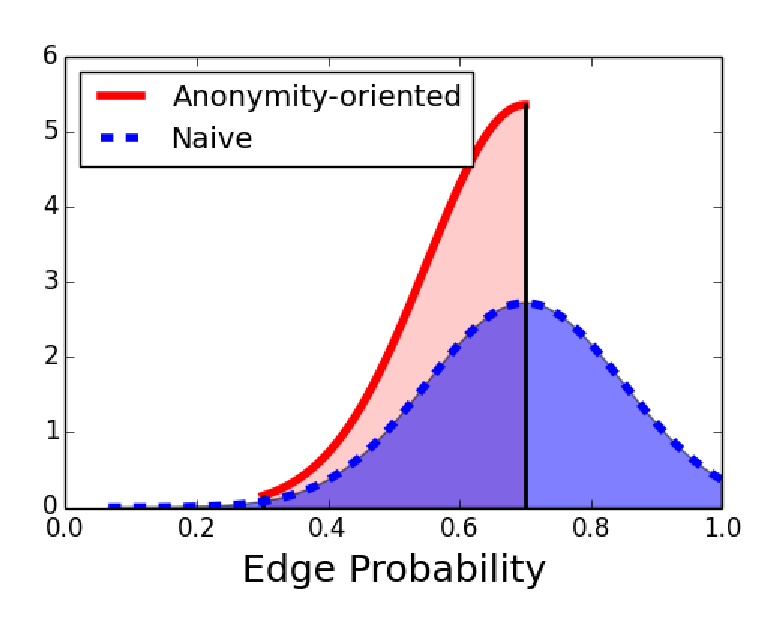
\includegraphics[width=1\textwidth]{ill/anonymityEP.eps}
    \end{minipage}
  }
  \subfigure[]{\label{fig:constraintRelax}  %(22)
    \begin{minipage}[l]{0.45\columnwidth}
      \centering
      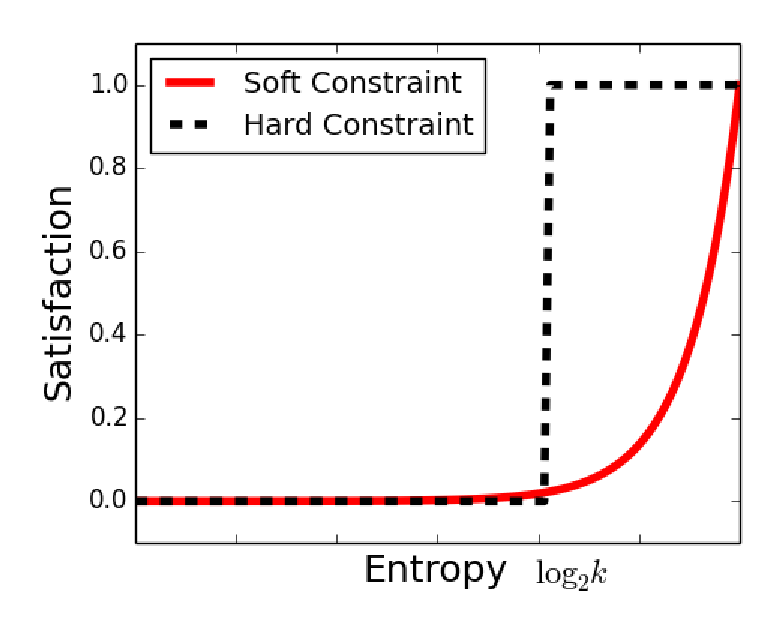
\includegraphics[width=1\textwidth]{ill/constraint.eps}
    \end{minipage}
  }
    \vspace{-0.7em}
    \caption{(a) Anonymity-oriented edge perturbing; (b) Relaxing $k$-obfuscation constraint.}
    \vspace{-1.5em}
\end{figure}






\subsubsection{Proof Sketching the Heuristic}
\label{sec:prooooof}
% {\todo{I still think this section is too detailed and no one will read such theorems and proofs, especially near the end of the paper. If that is not the formal proof, then the formal proof is what?? I would suggest describing the rational only here possibly with some figure and example...}}

We proceed to elaborate the rationality this anonymity-oriented edge perturbing scheme briefly. The formal detail proof of our heuristic is available in tech report. The core idea is to maximize the entropy of degree uncertainty matrix (referred to as ME). 

To facilitate further discussion, we consider the extreme case $k$-obf, which poses a set of hard constraints over the anonymized solution. Let the constraint being $k$-obf be $\mathbb{C}$, $k-$obfuscate a vertex $v$ be $\mathtt{c}_{v}$. 
According to Definition~\ref{def:obf}, $k-$obf can be expressed as joint satisfaction of $\lbrace c_{v}~:~v \in V \rbrace$ since the uncertain graph is said to be $k$-obf iff it $k-$obfuscates all the vertices. The formal definition as follows. 
\begin{equation}
    \mathbb{C}= \prod_{v \in V} \mathtt{c}_{v}
\end{equation}
where
\begin{equation*}
        \mathtt{c}_{v}:=
        \begin{cases}
                1  & H(Y_{P(v)}) \geq \log_{2}{k} \\
                0  & otherwise \\
         \end{cases}
\end{equation*}
In other words, given an uncertain graph, its satisfaction evaluation of $\mathbb{C}$ indicates whether it achieves the desirable anonymity level ($k$-obf).

However, as shown in Figure~\ref{fig:constraintRelax}, a single constraint at the vertex level is either fully satisfied or fully violated. It limits the optimization opportunity of methods based on local search. In this work, we model the individual constraint $c_{v}$ to a fuzzy relation in which the satisfaction of a constraint is a continuous function of its variables' values 
% ({\ie}, edge probabilities),  wrong statement 
({\ie}, the entropy $H(Y_{P(v)}$),
going from fully satisfied to fully violated as follows. 
\begin{equation}
    C_{v} = e^{H(Y_{P(v)})-\log_{2}{|V|}}
    \label{eq:approximate}
\end{equation}

\begin{lemma}
Let $\Omega$ presents the domain of degree values in the original uncertain graph, the maximization of the provided anonymity $\mathbb{C}$ is equivalent to the maximization of the following function:
  \begin{equation}
      \sum_{\omega \in \Omega} s(\omega) \cdot H(Y_{\omega}) 
      \label{eq:anonymity}
  \end{equation} 
\end{lemma}

{\bf Proof Sketch:} First we can see that 
\begin{align*}
    \mathcal{C} &= \prod_{v \in V} \mathtt{c}_{v} 
                 = \prod_{\omega \in \Omega} \underbrace{\mathtt{c_{\omega}} \ldots \mathtt{c}_{\omega}}_{s(\omega)} 
\end{align*}
Taking logarithm for both sides and combining with the approximation equation~\ref{eq:approximate}, we can see that 
\begin{align*}
    \log(\mathcal{C}) &=\sum_{\omega \in \Omega} s(\omega) \log(\mathtt{c_{\omega}}) \\
                      &=\sum_{\omega \in \Omega} s(\omega) \big[ H(Y_{\omega})-\log_{2}{|V|} \big] \\
                      &=\sum_{\omega  \in \Omega} s(\omega) H(Y_{\omega}) -\sum_{\omega  \in \Omega} \log_{2}{|V|}
\end{align*}
Therefore, after removing the constant $\sum_{\omega} \log_{2}|V|$ from $\log(\mathcal{C})$, our goal is actually to maximize Equation~\ref{eq:anonymity}. It provides us with the relation between the global anonymity and the level of disorder of the degree uncertainty matrix.  

% option a: use lemma with number, cross reference can be graceful 
\begin{lemma}
The maximization of Equation~\ref{eq:anonymity} is equivalent to maximization of the following function:
  \begin{equation}
      \small{\sum_{\omega \in \Omega} s(\omega) \cdot H(Y_{\omega}) =\big[ \sum_{v \in V} H(d_{v})\big] + |V|\log{|V|}-|V|H(\Omega)}
  \end{equation}
The equation stems from the coding length of degree uncertainty matrix from different perspectives (row and column).
% \footnote{More detail of it is available in tech report.}
\end{lemma}
It provides us with the mechanism for gaining better anonymity, namely increasing the degree uncertainty per vertex $H(d_{v})$. 

\begin{lemma}
As implied by the Central Limit Theorem, $d_{v}$ may be approximated by the normal distribution $\mathcal{N}(\mu,\sigma^2)$, where $\mu=\sum_{e \in \mathcal{E}^{v}} p(e)$ and $\sigma^2=\sum_{e \in \mathcal{E}^{v}} p(e)-p(e)^2$. Therefore, its entropy may be approximated by the differential entropy of the normal distribution $\frac{1}{2} \ln(2\pi\sigma^2) + \frac{1}{2}$. For a given $p(e)$, its gradient ascent is proportion to $1-2\cdot p(e)$. 
\end{lemma}
Targeting at high entropy, we apply the gradient ascent method---$\hat{p}(e)=p(e)+ \big( 1-2\cdot p(e) \big) \cdot r_{e} $ for achieving the increase of degree entropy and the anonymity gain.
